\scanpage{10}
% archive sheet number: 9
(4.3) est connu pour tout $G$ par la seule connaissance de
\[
\mathrm{R}f_{\handwritten{!}}(A_X(d-d')\handwritten{[}2(d-d')\handwritten{]})\handwritten{\longrightarrow}A_Y.
\tag*{(4.4)}
\]
Ceci devrait bien donner la formule de projection au niveau des classes de cohomologie (qu'il faut bien entendu expliciter, soit ici, soit\inserted{(mieux)} à la fin du formulaire, en reprenant ce formulaire dans \deleted{\unsure{le ca}} le cas particulier recommandé\handwritten{,} parmi les variantes possibles).

\deleted{\unsure{b}}\handwritten{a}) \uline{Si} $d=d'$ \uline{et si} $\unsure{g|f}$ \uline{est quasi-fini} (et alors automatiquement plat, supposant que la dimension relative de $p$ est partout $d$), alors on retrouve l'homomorphisme trace de XVII ...

\deleted{\unsure{c}}\handwritten{b}) Si $f$ \uline{est lisse}, on retrouve l'homomorphisme trace du par.2.

\deleted{\unsure{d}}\handwritten{c}) \uline{Transitivité} pour un composé $gf$ ($g:Y\handwritten{\longrightarrow}Z$, avec $Z$ lisse et compactifiable sur $S$).

\margin{\handwritten{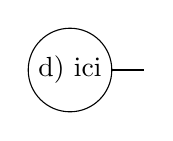
\begin{tikzpicture}\node[draw,circle,inner sep=2pt] (n) {d) ici};\draw (n.east)--++(0.4,0);\end{tikzpicture}}}
\deleted{\unsure{e}}\handwritten{f}) Compatibilité avec \uline{Künneth}, quand on regarde $g_1\mathbin{\mathrm{x}}_S g_2:X_1\mathbin{\mathrm{x}}_S X_2\handwritten{\longrightarrow}Y_1\mathbin{\mathrm{x}}_S Y_2$. Compatibilité avec \uline{changement de base}\inserted{$S'\handwritten{\longrightarrow}S$.}

\deleted{\unsure{f}}\handwritten{e}) Compatibilité avec \uline{changement d'Anneau} $A\handwritten{\longrightarrow}A'$ (qui \unsure{montre} qu'il suffit de connaitre (4.4) pour les $A=(\underline{\mathrm{Z}}/n\underline{\mathrm{Z}})_S$ pour l'avoir pour tout $A$).

 g) \uline{Indépendance par rapport à} $S$ (si on se donne $S\handwritten{\longrightarrow}\deleted{\unsure{S|et}}T$ lisse, de sorte que l'on peut regarder $X$ et $Y$ comme étant sur $T$ ...).

 h) \uline{Formule d'échange}, relatif au cas où on a un diagramme cartésien
\diagram{\begin{tikzcd}[ampersand replacement=\&,row sep=2em,column sep=2em,execute at end picture={\draw[gray] ([xshift=-2pt,yshift=6pt]xx.north west) .. controls ([xshift=-22pt,yshift=10pt]xx.west) and ([xshift=-18pt,yshift=-14pt]yy.west) .. ([yshift=-12pt]yy.south) .. controls ([xshift=25pt,yshift=-16pt]yyp.south) and ([xshift=20pt,yshift=12pt]yyp.east) .. ([yshift=12pt]yyp.north) .. controls ([xshift=-10pt,yshift=20pt]yyp.north) and ([yshift=-14pt]xx.east) .. ([xshift=9pt]xx.north east);}]
|[alias=xx]| X \handwritten{\arrow[d,"f"']} \& X' \handwritten{\arrow[l,"h"']} \handwritten{\arrow[d,"f'"]} \\
|[alias=yy]| Y \& |[alias=yyp]| Y' \handwritten{\arrow[l,"g"']}
\end{tikzcd}}
de schémas sur $S$: appliquant $g^*$ à $\mathrm{Tr}_f$, et appliquant \deleted{\unsure{la for}} l'isomorphisme de changement de base pour $\mathrm{R}f_{\handwritten{!}}$ et $g^*$, on doit trouver $\mathrm{Tr}_{f'}$. On supposera bien sûr $Y$ et $Y'$ lisses sur $S$, $X$ plat sur $S$, et pour que $X'$ soit plat sur $S$, il faut évidemment une hypothèse genre Tor-indépendance de $X$ et $Y'$ sur $Y$. Cela doit marcher en tous cas si $X$ est également lisse sur $S$, et si $f$ et $g$ sont \uline{transversaux} (EGA IV \unsure{17|27}...).
